\chapter{Test Setups}
\label{chap:\currfilebase}

\subsection{Hammer-Hammer Test}

The hammer tips of the reference system and the experimental system are hit against eachother.
\begin{figure}[!htb]
    \centering
    \includestandalone[scale=1]{\imgpath/test_setups/HH_parts/HH_parts}
    \\[0.5em]
    \footnotesize
		\begin{tabular}{c@{ :\hskip 0.5em}l}
			\toprule
            \large{1} & Piezo + \ac{AMP}\\
            \large{2} & Soft Tip\\
            \large{3} & Tip 34CrMo4\\
            \large{4} & \ac{LC} DYMH-103\\
            \large{5} & \ac{IN-AMP} AD627\\
			\bottomrule
		\end{tabular}
	\normalsize
    \caption[MCU communication protocol]{Protocol used to communicate between two MCU's and between MCU and computer}
    \label{tab:mcu_com_protocol}
\end{figure}

\begin{figure}[!htb]
    \centering
    \includestandalone[width=0.9\linewidth]{\imgpath/test_setups/HH_comparison/HH_comparison}
    \caption[HH-Test comparison]{The HH-Test recordings of the reference hammer (orange) and the evaluated impact hammer system (turquoise). Note that the evaluated signal values are normalized so that the maxima are equal to the reference system.}
    \label{tab:mcu_com_protocol}
\end{figure}
\begin{figure}[!htb]
    \centering
    \includestandalone[width=\linewidth]{\imgpath/test_setups/HH_noise/HH_noise}
    \caption[HH-Test comparison]{The HH-Test recordings of the reference hammer (orange) and the evaluated impact hammer system (turquoise). Note that the evaluated signal values are normalized so that the maxima are equal to the reference system.}
    \label{fig:HH_noise}
\end{figure}

\subsection{Andromeda FRF measurement}

\begin{figure}[!htb]
    \centering
    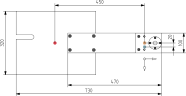
\includegraphics[scale=1]{\imgpath/test_setups/Andromeda/Andromeda_Positions_Top}
    \caption[Andromeda Positions Top View]{Andromeda}
    \label{Andromeda_Positions_Top}
\end{figure}

\begin{figure}[!htb]
    \centering
    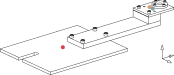
\includegraphics[scale=1]{\imgpath/test_setups/Andromeda/Andromeda_Positions_Trimetric_coord}
    \caption[Andromeda Positions Trimetric View]{Andromeda}
    \label{Andromeda_Positions_Trimetric_coord}
\end{figure}

\begin{figure}[!htb]
    \centering
    \includegraphics[width=0.5\linewidth]{\imgpath/test_setups/Andromeda/Andromeda_Sensors.jpg}
    \caption[Andromeda Positions Sensors View]{Andromeda}
    \label{Andromeda_Sensors}
\end{figure}

% \begin{figure}[!htb]
%     \centering
%     \includegraphics[width=0.5\linewidth]{\imgpath/test_setups/Andromeda/Andromeda_total.jpg}
%     \caption[Andromeda Overview]{Andromeda_total}
%     \label{Andromeda_total}
% \end{figure}